% TODO Adjust the title to match the one we specified in the application.

\documentclass{beamer}

\usepackage{amsmath,amssymb,amsfonts}
\usepackage{array}
\usepackage[british]{babel}
\usepackage{bbm}
\usepackage{bbold}
\usepackage{beamerthemesplit}
\usepackage[bf]{caption}
\usepackage{cite}
\usepackage{color}
\usepackage{enumerate}
\usepackage{eurosym}
\usepackage{graphicx}
\usepackage{rotating}
\usepackage{slashed}
\usepackage[utf8]{luainputenc}
\usepackage{xcolor}
\usepackage{array}
\usepackage{listings}

\usepackage{pgfplots}
\pgfplotsset{compat=1.10}

% My fonts:
% ---------
\usepackage{libertine}
\usefonttheme[onlymath]{serif}

\usepackage[activate]{microtype}

%----------------------------------------------------------------------------------------
% C++ STYLES
%----------------------------------------------------------------------------------------

\definecolor{codegreen}{rgb}{0,0.6,0}
\definecolor{codegray}{rgb}{0.5,0.5,0.5}
\definecolor{codepurple}{rgb}{0.58,0,0.82}
\definecolor{backcolour}{rgb}{0.95,0.95,0.92}
\lstdefinestyle{mystyle}{
	language=C++,
  % backgroundcolor=\color{backcolour},
  commentstyle=\color{codegreen},
  keywordstyle=\color{magenta},
  numberstyle=\tiny\color{codegray},
  stringstyle=\color{codepurple},
  basicstyle=\tiny\ttfamily,
  breakatwhitespace=false,
  breaklines=true,
  captionpos=b,
  keepspaces=true,
  % numbers=left,
  numbersep=5pt,
  showspaces=false,
  showstringspaces=false,
  showtabs=false,
  tabsize=2,
        keywords={var, func, extends},
}
\lstset{style=mystyle}

%----------------------------------------------------------------------------------------
% OTHER STUFF
%----------------------------------------------------------------------------------------

\DeclareMathOperator{\tr}{tr}
\makeatletter
\def\amsbb{\use@mathgroup \M@U \symAMSb}
\makeatother

\usetheme{Boadilla}

\setbeamertemplate{section in toc}[sections numbered]
\setbeamertemplate{blocks}[rounded][shadow=false]
\setbeamertemplate{itemize items}[default]
\beamertemplatenavigationsymbolsempty
\setbeamercolor{footline}{bg=black}
\setbeamertemplate{footline}{%
  \raisebox{8pt}{\makebox[\paperwidth]{\hfill\makebox[15pt]{{\tiny\insertframenumber}}\qquad}}
}

\definecolor{myred}{RGB}{176,50,50}
\definecolor{myblue}{RGB}{50,50,176}
\definecolor{mygreen}{RGB}{60,166,60}

\newcommand\blfootnote[1]{%
  \begingroup
    \renewcommand\thefootnote{}\footnote{#1}%
    \addtocounter{footnote}{-1}%
    \endgroup
}

%\usepackage{pgfpages}
%\setbeameroption{show notes on second screen}


\begin{document}

\allowdisplaybreaks[1]

\title{Lattice QCD Stencils on Intel Xeon Phis}
\author{Peter Labus \and Martin Ueding \\[2ex] University of Bonn, Germany}
  \date{Cineca \\ 03/23/2017}

  %%%%%%%%%%%%%%%%%%%%%%%%%%%%%%%%%%%%%%%%%%
  %%%   TITLE SLIDE
  %%%%%%%%%%%%%%%%%%%%%%%%%%%%%%%%%%%%%%%%%%

  \begin{frame}
    \titlepage
  \end{frame}

  %%%%%%%%%%%%%%%%%%%%%%%%%%%%%%%%%%%%%%%%%%
  %%%   SLIDE 1
  %%%%%%%%%%%%%%%%%%%%%%%%%%%%%%%%%%%%%%%%%%

  \setcounter{framenumber}{0}

  \begin{frame}
    \frametitle{LQCD \& the r\^ole of the \textit{dslash} stencil}

    \begin{itemize}
      \item  Calculate integrals of the form
        \begin{align*}
          \int \mathcal D \Phi \; f[\Phi] \, \mathrm e^{-S_\text{QCD}[\Phi]}
        \end{align*}
        after \textit{discretising} space-time through a lattice
        \vfill

      \item Algorithmic layers of LQCD:
        \begin{enumerate}
          \item Hybrid Monte Carlo
          \item Efficient Krylov Solvers for $Mx=b$ in Molecular Dynamics
          \item BLAS linear algebra
        \end{enumerate}
        \vfill

      \item Most \textit{expensive} part:\\[1mm]
        \hspace{2mm} Matrix times Vector (very large \& sparse),\\
        \hspace{2mm} described by \textbf{nearest-neighbour stencil}
        \vfill
    \end{itemize}

  \end{frame}

  %%%%%%%%%%%%%%%%%%%%%%%%%%%%%%%%%%%%%%%%%%
  %%%   SLIDE 2
  %%%%%%%%%%%%%%%%%%%%%%%%%%%%%%%%%%%%%%%%%%

  \begin{frame}
    \frametitle{The QPhiX library (mainly: Bálint Joó, Jefferson Lab)}

    \begin{itemize}
      \item Aim: provide stencil operations for \textbf{general vector machines}
        \vfill
      \item Parallelised via QMP + OpenMP + SIMD (vector intrinsics)
        \vfill
      \item C++11 template library with external C++ \textbf{code generator}\\
        ($\sim25k$ lines of code + $10k$ testing \& timing)
        \vfill
      \item Implements
        \begin{enumerate}
          \item Wilson / Wilson-Clover \textit{dslash} stencils
          \item BLAS linear algebra
          \item Krylov Solvers (CG, BiCGStab, Mixed Precision, MultiCG)
        \end{enumerate}
        \vfill
      \item Common template parameters:
        \begin{enumerate}
          \item \texttt{typename FT}
          \item \texttt{int VECLEN}
          \item \texttt{int SOALEN}
          \item \texttt{bool COMPRESS12}
        \end{enumerate}
        \vfill
    \end{itemize}

  \end{frame}

  %%%%%%%%%%%%%%%%%%%%%%%%%%%%%%%%%%%%%%%%%%
  %%%   SLIDE 3
  %%%%%%%%%%%%%%%%%%%%%%%%%%%%%%%%%%%%%%%%%%

  \begin{frame}
    \frametitle{The \textit{dslash} stencil in action}

    \begin{align*}
      \nonumber
      \chi^a_\alpha(x)
      % &= \sum_{y \in \Lambda} \sum_{b = 0}^2 \sum_{\beta = 0}^3 \slashed D^{ab}_{\alpha \beta}(x,y) \psi^b_\beta(y) \\
      &= \sum_{b = 1}^3 \sum_{\beta = 1}^4 \sum_{\mu=1}^4
      \bigg[
        U^{ab}(x,x+\hat\mu) \; P^{-\, \mu}_{\alpha\beta} \; \psi^b_\beta(x+\hat\mu) + \\
        \nonumber
        &\hspace{25.0mm}
        U^{\dagger\, ab}(x,x-\hat\mu) \; P^{+\,\mu}_{\alpha\beta} \; \psi^b_\beta(x-\hat\mu)
      \bigg]
    \end{align*}

    \vfill
    For each site $x$ of the lattice:
    \vfill
    \begin{enumerate}
      \item Project on \textit{half} the spinor components via $P^{\pm\,\mu}_{\alpha\beta}$
      \item Hermitian Matrix Multiplication ($3 \times 3$ complex)
      \item Reconstruct and accumulate 8 contributions
    \end{enumerate}
    % \begin{itemize}
    %   \item $x,y$: points/sites of the lattice $\Lambda$\\
    %   \item $\psi$: input \textbf{spinor}: $3 \times 4 \times 2 = 24$ components per site\\
    %   \item $\chi$: output spinor\\
    %   \item $U$: \textbf{gauge} or link variables: $3 \times 3 \times 2 = 18$ components per site\\
    %   \item $\gamma_\mu$: 4 constant $4 \times 4$ complex matrices
    %   \item $\hat \mu$: 4 unit vectors (one for each space-time dimension)
    % \end{itemize}

  \end{frame}

  %%%%%%%%%%%%%%%%%%%%%%%%%%%%%%%%%%%%%%%%%%
  %%%   SLIDE 4
  %%%%%%%%%%%%%%%%%%%%%%%%%%%%%%%%%%%%%%%%%%

  \begin{frame}
    \frametitle{Arithmetic Intensities}
    \vspace{-5mm}
    \footnotesize

    \begin{align*}
      I_A = \textrm{FLOPs per Byte of moved data [here: single precision]}
    \end{align*}

    \begin{columns}[t]
    \begin{column}{0.49\linewidth}
      \begin{block}{Our Stencil Operations}
      \textbf{\textit{dslash} stencil:} \\ $\slashed D \,x$ \hfill 1320 FLOPs per site
      \begin{align*}
        I_A = 1.06 \; \textrm{FLOP/Byte}
      \end{align*}

      \textbf{\textit{dslash} stencil with clover term:} \\ $A^{-1}  \slashed D \, x$ \hfill 1872 FLOPs per site
      \begin{align*}
        I_A = 1.17 \; \textrm{FLOP/Byte}
      \end{align*}
      \end{block}
    \end{column}

    \hfill
    \begin{column}{0.49\linewidth}
      \begin{block}{The Hardware Peak}
      \textbf{Theoretical Peaks on KNL / KNC:}
      \begin{align*}
        I_A = 15.4 \, / \, 6.3 \; \textrm{FLOP/Byte}
      \end{align*}
      \vfill
      \end{block}
    \end{column}
    \end{columns}

    \vfill
    {
      \large
      \centering \textbf{All routines are memory bandwidth bound}\\
    }

    \vfill
    Combining these intensities with a simple hardware model and the (measured) memory bandwidth
    gives us a good \textit{rooftop model} \dots

  \end{frame}

  %%%%%%%%%%%%%%%%%%%%%%%%%%%%%%%%%%%%%%%%%%
  %%%   SLIDE 5
  %%%%%%%%%%%%%%%%%%%%%%%%%%%%%%%%%%%%%%%%%%

  \begin{frame}
    \frametitle{Intel Xeon Phi Knights Landing Hierarchies}

    \begin{columns}[T]
      \begin{column}{.5\textwidth}
        \vspace{3mm}
        {
          \center Peak Performance versus
          Memory Bandwidth:
        }
        \vspace{3mm}
        \begin{itemize}
          \item up to 72 cores @ 1.5 GHz\\ (3.5 TFLOP/s)
          \item 2D Mesh: 700 GB/s
          \item 8 GB MCDRAM: 450 GB/s
          \item 384 GB DDR-4: 90 GB/s
        \end{itemize}
      \end{column}
      \begin{column}{.5\textwidth}
        \begin{center}
          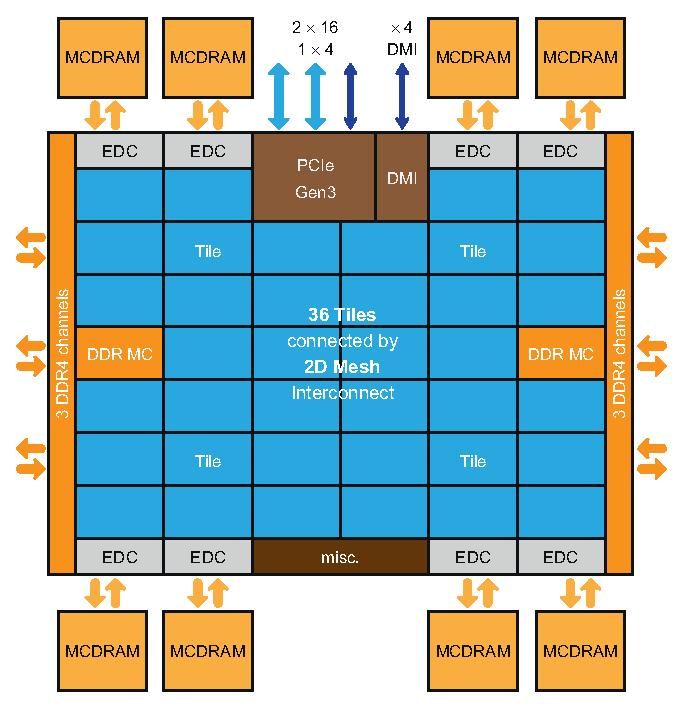
\includegraphics[width=0.9\textwidth]{knl.eps}
        \end{center}
      \end{column}
    \end{columns}

  \end{frame}

  %%%%%%%%%%%%%%%%%%%%%%%%%%%%%%%%%%%%%%%%%%
  %%%   SLIDE 6
  %%%%%%%%%%%%%%%%%%%%%%%%%%%%%%%%%%%%%%%%%%

  \begin{frame}
    \frametitle{General Programming Implications}

    Three Guidelines...
    \begin{enumerate}
      \item \textbf{Scaling}
      \item \textbf{Vectorisation}
      \item \textbf{Data Locality \& Cache Re-use}
    \end{enumerate}
    \vfill

    ... and how they are implemented in QPhiX
    \begin{enumerate}
      \item \textbf{OpenMP thread scheduling} for lattice traversal
      \item Multi-ISA \textbf{C++ code generator} using Vector Intrinsics
      \item \textbf{Cache blocking} into L2 and \textbf{Structures of Arrays} data layout (\textit{tiles})
    \end{enumerate}
    \vfill

    \textbf{Optimisations in QPhiX-codegen:}\\
    L1 \& L2 software prefetches,
    dimensions of tiles (\texttt{SOALEN}),\\
    streaming stores, gather/scatter instructions, \dots

  \end{frame}

  %%%%%%%%%%%%%%%%%%%%%%%%%%%%%%%%%%%%%%%%%%
  %%%   SLIDE 7
  %%%%%%%%%%%%%%%%%%%%%%%%%%%%%%%%%%%%%%%%%%

  \begin{frame}
    \frametitle{Data layout \& Cache blocking}

    \begin{itemize}
      \item Elementary vector elements are \textit{Structures of Arrays} (SoA):\\
        \texttt{typedef FT FourSpinorBlock[3][4][2][SOALEN];}
        \vfill

      \item \texttt{SOALEN} may be a factor of $\texttt{VECLEN} = \texttt{ngy} * \texttt{SOALEN}$:\\
        form \textit{tiles} in X-Y-plane (Xeon Phi SP: $16\times1$, $8\times2$, $4\times4$)
    \end{itemize}

    \begin{columns}

      \begin{column}{.4\textwidth}
        \begin{center}
          \begin{itemize}
            \item Then divide lattice in blocks:
              \begin{description}
                \item[X]    \texttt{SOALEN}\\
                \item[Y, Z] \texttt{By}, \texttt{Bz}\\[2mm]
              \end{description}
              such that 3 T-Slices fit into L2
              \vfill
          \end{itemize}
        \end{center}
      \end{column}

      \begin{column}{.6\textwidth}
        \begin{center}
\begin{tikzpicture}[scale=0.3]

    \fill[fill=black!20] (0, 0) rectangle +(8, 1);
    \fill[fill=black!10] (0, 1) rectangle +(8, 1);

    \draw[dotted] (0, 0) grid (16, 8);

    \draw[black!30, xstep=4, ystep=2] (0, 0) grid (16, 8);

    \draw[thick, xstep=4, ystep=4] (0, 0) grid (16, 8);
    \draw[thick] (0, 0) rectangle (16, 8);

    \draw[|-|] (0, -0.5) -- (4, -0.5) node[below, midway] {\texttt{soalen}};
    \draw[|-|] (-0.5, 0) -- (-0.5, 2) node[left, midway] {\texttt{ngy}};
    \draw[|-|] (-0.5, 4) -- (-0.5, 8) node[left, midway] {\texttt{By}};
    \draw[|-|] (16.5, 0) -- (16.5, 8) node[right, midway] {\texttt{Ly}};
    \draw[|-|] (0, 8.5) -- (16, 8.5) node[above, midway] {\texttt{Lx}};

          \end{tikzpicture}
        \end{center}
      \end{column}

    \end{columns}

  \end{frame}

  %%%%%%%%%%%%%%%%%%%%%%%%%%%%%%%%%%%%%%%%%%
  %%%   SLIDE 8
  %%%%%%%%%%%%%%%%%%%%%%%%%%%%%%%%%%%%%%%%%%

  \begin{frame}
    \frametitle{Heuristic Load Balancing}


    \begin{columns}
      \begin{column}{.45\linewidth}
        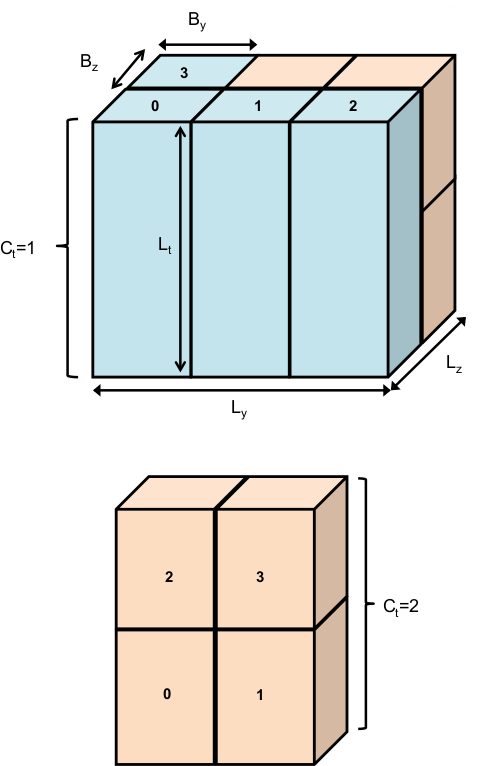
\includegraphics[height=0.85\textheight]{phases-crop.png}
      \end{column}
      \begin{column}{.50\linewidth}
        3.5 Dimensional Blocking:

        \begin{itemize}
          \item Each core processes one block per phase
          \item If fewer blocks than core, split in T-direction
          \item Process remainder after maximum number of splits
        \end{itemize}
      \end{column}
    \end{columns}

  \end{frame}

  %%%%%%%%%%%%%%%%%%%%%%%%%%%%%%%%%%%%%%%%%%
  %%%   SLIDE 9
  %%%%%%%%%%%%%%%%%%%%%%%%%%%%%%%%%%%%%%%%%%

  \begin{frame}
    \frametitle{QPhiX-codegen}

    \begin{itemize}

      \item Three abstract classes:
        \begin{enumerate}
          \item \texttt{Instruction}
          \item \texttt{Address}
          \item \texttt{FVec}
        \end{enumerate}
        \vfill

      \item First two classes: \;\; \texttt{std::string serialize(void)}
        \vfill

      \item Concrete implementations of \texttt{serialize} determine the ISA\\

    \lstinputlisting[language=C++, basicstyle=\footnotesize\ttfamily]{fma-avx512.cpp}

        \vfill

      \item Save Instructions into \texttt{InstVector}'s and dump to file

    \end{itemize}

  \end{frame}

  %%%%%%%%%%%%%%%%%%%%%%%%%%%%%%%%%%%%%%%%%%
  %%%   SLIDE 10
  %%%%%%%%%%%%%%%%%%%%%%%%%%%%%%%%%%%%%%%%%%

  \begin{frame}[fragile]
    \frametitle{Code Example: Hermitian Matrix Multiplication}
    \small

    \lstinputlisting[language=C++]{clover.cc}
\end{frame}

  %%%%%%%%%%%%%%%%%%%%%%%%%%%%%%%%%%%%%%%%%%
  %%%   SLIDE 13
  %%%%%%%%%%%%%%%%%%%%%%%%%%%%%%%%%%%%%%%%%%

  \begin{frame}
    \frametitle{Optimisation Features}


    \begin{block}{Code Generator}
    \begin{itemize}
        \item L1 Prefetches
        \item L2 Prefetches
        \item Streaming Stores
        \item Gauge Packing
        \item Barriers
    \end{itemize}
    \end{block}

    \begin{block}{QPhiX}
    \begin{itemize}
      \item Floating point type
      \item SoA length
      \item Gauge Compression
    \end{itemize}
    \end{block}

  \end{frame}

  \begin{frame}
    \frametitle{Optimisation Features on KNC vs. KNL}
    \footnotesize

    {\tiny
    Displayed is the basic \textit{dslash} stencil ($c_{sw}=\mu=0$) in single precision
    with $\texttt{SOA}=16$.}

    \begin{columns}[T]
      \begin{column}{.5\textwidth}
        \begin{center}
          KNC:\\
      \begin{tikzpicture}[scale=0.6]
        \begin{axis}[
            xtick=data,
            xticklabels={
vector + packed + streaming,
           + L1,
           + L2,
           + L1 and L2,
+ Barrier,
+ SOA=8,
+ compression
            },
            x tick label style={rotate=-35,anchor=north west},
                  ylabel={GFlop/s},
                  ymin=0,
                  ymax=470,
                  ybar,
                  legend pos=outer north east,
                  ymajorgrids=true,
                ]

              \addplot coordinates
              {
                (1, 172)
                (2, 144)
                (3, 176)
                (4, 191)
                (5, 199)
                (6, 234)
                (7, 286)
              };

        \end{axis}
      \end{tikzpicture}

          \vfill
        \end{center}
      \end{column}
      \begin{column}{.5\textwidth}
        \begin{center}
          KNL (DEEP):\\
      \begin{tikzpicture}[scale=0.6]
        \begin{axis}[
            xtick=data,
            xticklabels={
vector,
+ packed gauges,
+ streaming stores,
(3) + L1,
(3) + L2,
(3) + L1 and L2,
(3) + Barrier,
+ SOA=8,
+ compression,
            },
            x tick label style={rotate=-35,anchor=north west},
                  ylabel={GFlop/s},
                  ymin=0,
                  ymax=470,
                  ybar,
                  legend pos=outer north east,
                  ymajorgrids=true,
                ]

              \addplot+[error bars/.cd, y dir=both, y explicit] coordinates
              {
                (1, 362.5) +- (0, 18.4)
                (2, 384.3) +- (0, 19.3)
                (3, 380.1) +- (0, 18.6)
                (4, 377.5) +- (0, 18.6)
                (5, 344.9) +- (0, 14.3)
                (6, 359.5) +- (0, 13.5)
                (7, 381.2) +- (0, 26.9)
                (8, 386.9) +- (0, 21.0)
                (9, 434.2) +- (0, 14.5)
              };

        \end{axis}
      \end{tikzpicture}
        \end{center}
      \end{column}
    \end{columns}

    \begin{itemize}
      \item KNL natively supports prefetches \& streaming stores much better than KNC
        \vfill
      \item Visible benefits from data layout tuning (shown here: SoA length tuning)
        \vfill
      % \item greatest benefits from algorithmic improvements
    \end{itemize}

  \end{frame}

  \begin{frame}
    \frametitle{Single Node Performance}

      \begin{columns}[t]
        \begin{column}{0.4\linewidth}
          \begin{tikzpicture}
            \begin{axis}[
                title=DEEP,
                width=\linewidth,
                height=0.5\textheight,
                xmin=1.5,
                xmax=3.5,
                ymin=0,
                ymax=470,
                xtick={2, 3},
                xticklabels={4, 8},
                xlabel={SoA length},
                ylabel={GFlop/s},
                ybar,
                ymajorgrids=true,
              ]

              \addplot+[error bars/.cd, y dir=both, y explicit] coordinates {
                ( 2.0, 299.804833333) +- (0, 10.4998327882)
                ( 3.0, 437.045666667 ) +- (0, 9.28507893846) };
              \addplot+[error bars/.cd, y dir=both, y explicit] coordinates {
                ( 2.0, 371.738) +- (0, 6.58345238394)
                ( 3.0, 421.222) +- (0, 5.61352336748) };

            \end{axis}
          \end{tikzpicture}
        \end{column}

        \begin{column}{0.6\linewidth}
          \begin{tikzpicture}
            \begin{axis}[
                title=Marconi A2,
                width=0.7\linewidth,
                height=0.5\textheight,
                xmin=1.5,
                xmax=3.5,
                ymin=0,
                ymax=470,
                xtick={2, 3},
                xticklabels={4, 8},
                xlabel={SoA length},
                ybar,
                legend pos=outer north east,
                ymajorgrids=true,
              ]

              \addplot+[error bars/.cd, y dir=both, y explicit] coordinates {
                ( 2.0 , 217.841833333) +- (0, 0.993589751813)
                ( 3.0 , 363.165083333) +- (0, 2.7395950569) };
              \addlegendentry{ Half }
              \addplot+[error bars/.cd, y dir=both, y explicit] coordinates {
                ( 2.0 , 306.195333333) +- (0, 1.95385987405)
              ( 3.0 , 315.29625) +- (0, 1.86925662633) };
              \addlegendentry{ Single }
              \addplot+[error bars/.cd, y dir=both, y explicit] coordinates {
                ( 2.0 , 122.167083333) +- (0, 0.678511273327)
              ( 3.0 , 114.3745) +- (0, 0.753930501697) };
              \addlegendentry{ Double }

            \end{axis}
          \end{tikzpicture}
        \end{column}
      \end{columns}

          One KNL, one MPI rank, $64 \times 4$ threads, $L = 48$, $T = 96$

      %Half prec is not faster in hardware, is good for bandwidth limited programs (like ours)
    \end{frame}

  \begin{frame}
      \frametitle{Multi Node Performance}
      \framesubtitle{Parameters}

      \begin{itemize}
          \item SOALEN = 8
          \item Block size = 4
          \item Single precision
          \item 12-Parameter gauge compression
          \item Lattice sizes $32^3 \times 64$, $48^3 \times 96$, and $64^3 \times 128$
          \item Error bar denotes standard error with 12 repetitions
      \end{itemize}

      \begin{itemize}
          \item Cache mode
          \item Quadrant configuration
          \item One MPI rank per KNL, using 68 threads
          \item 8, 16, 32, and 64 KNL
          \item Different rank geometries ($g_1 g_2 g_3 g_4 = \text{\# ranks}$)
          \item Runs performed 2017-03-14 (last Tuesday)
      \end{itemize}

  \end{frame}

  \begin{frame}
      \frametitle{Multi Node Performance}
      \framesubtitle{Strong Scaling}

      \begin{columns}
        \begin{column}{0.5\linewidth}
             
      \begin{tikzpicture}
          \begin{axis}[
              title=JURECA,
              width=\linewidth,
              height=0.6\textheight,
                  xmin=0,
                  ymin=0,
                  xlabel={Number of Nodes},
                  ylabel={TFlop/s Total},
                  %legend pos=outer north east,
                  grid=major,
              ]
              \addplot+[only marks, mark=*, error bars/.cd, y dir=both, y explicit]
              table[y error index=2] {jureca-strong-64.tsv};
              %\addlegendentry{$L = 64$}
              \addplot+[only marks, mark=*, error bars/.cd, y dir=both, y explicit]
              table[y error index=2] {jureca-strong-48.tsv};
              %\addlegendentry{$L = 48$}
              \addplot+[only marks, mark=*, error bars/.cd, y dir=both, y explicit]
              table[y error index=2] {jureca-strong-32.tsv};
              %\addlegendentry{$L = 32$}
          \end{axis}
      \end{tikzpicture}

         \end{column}
        \begin{column}{0.5\linewidth}
             
      \begin{tikzpicture}
          \begin{axis}[
              title=Marconi A2,
              width=\linewidth,
              height=0.6\textheight,
                  xmin=0,
                  ymin=0,
                  xlabel={Number of Nodes},
                  %ylabel={GFlop/s Total},
                  %legend pos=outer north east,
                  grid=major,
                  xtick=data,
              ]
              \addplot+[only marks, mark=*, error bars/.cd, y dir=both, y explicit]
              table[y error index=2] {strong-64.tsv};
              %\addlegendentry{$L = 64$}
              \addplot+[only marks, mark=*, error bars/.cd, y dir=both, y explicit]
              table[y error index=2] {strong-48.tsv};
              %\addlegendentry{$L = 48$}
              \addplot+[only marks, mark=*, error bars/.cd, y dir=both, y explicit]
              table[y error index=2] {strong-32.tsv};
              %\addlegendentry{$L = 32$}
          \end{axis}
      \end{tikzpicture}

         \end{column}
      \end{columns}
      
        \vfill

      Lattice sizes: Blue 64, Red 48, Gold 32.

  \end{frame}

  \begin{frame}
      \frametitle{Multi Node Performance}
      \framesubtitle{Weak Scaling}

      \begin{columns}
        \begin{column}{0.5\linewidth}
            
      \begin{tikzpicture}
          \begin{axis}[
              title=JURECA,
              width=\linewidth,
              height=0.6\textheight,
                  xmin=0,
                  ymin=0,
                  xlabel={Number of Nodes},
                  ylabel={GFlop/s per Node},
                  %legend pos=outer north east,
                  grid=major,
              ]
              \addplot+[only marks, mark=*, error bars/.cd, y dir=both, y explicit]
              table[y error index=2] {jureca-weak-64.tsv};
              %\addlegendentry{$L = 64$}
              \addplot+[only marks, mark=*, error bars/.cd, y dir=both, y explicit]
              table[y error index=2] {jureca-weak-48.tsv};
              %\addlegendentry{$L = 48$}
              \addplot+[only marks, mark=*, error bars/.cd, y dir=both, y explicit]
              table[y error index=2] {jureca-weak-32.tsv};
              %\addlegendentry{$L = 32$}
          \end{axis}
      \end{tikzpicture}
        \end{column}

        \begin{column}{0.5\linewidth}
            
      \begin{tikzpicture}
          \begin{axis}[
              title=Marconi A2,
              width=\linewidth,
              height=0.6\textheight,
                  xmin=0,
                  ymin=0,
                  xlabel={Number of Nodes},
                  %ylabel={GFlop/s per Node},
                  %legend pos=outer north east,
                  grid=major,
                  xtick=data,
              ]
              \addplot+[only marks, mark=*, error bars/.cd, y dir=both, y explicit]
              table[y error index=2] {weak-64.tsv};
              %\addlegendentry{$L = 64$}
              \addplot+[only marks, mark=*, error bars/.cd, y dir=both, y explicit]
              table[y error index=2] {weak-48.tsv};
              %\addlegendentry{$L = 48$}
              \addplot+[only marks, mark=*, error bars/.cd, y dir=both, y explicit]
              table[y error index=2] {weak-32.tsv};
              %\addlegendentry{$L = 32$}
          \end{axis}
      \end{tikzpicture}
        \end{column}
          
      \end{columns}

      
        \vfill

      Lattice sizes: Blue 64, Red 48, Gold 32.
  \end{frame}

  \begin{frame}
    \frametitle{Benefit for Xeon}

    \begin{columns}
      \begin{column}{0.5\linewidth}
          \begin{tikzpicture}
            \begin{axis}[
                title={Solve},
                width=\linewidth,
                %height=0.3\textheight,
                ymin=0,
                xmin=0.5,
                xmax=2.5,
                xtick={1, 2},
                xticklabels={Chroma, QPhiX},
                xlabel={Implementation},
                ylabel={Seconds},
                ybar,
                ymajorgrids=true,
                ytick=data,
              ]

              \addplot coordinates {
                ( 1.0 , 6.073364 )
                ( 2.0 , 0.590205 )
              };


            \end{axis}
          \end{tikzpicture}

%          \begin{tikzpicture}
%            \begin{axis}[
%                title={Solve},
%                width=\linewidth,
%                height=0.3\textheight,
%                ymin=0,
%                xmin=0.5,
%                xmax=2.5,
%                xtick={1, 2},
%                xticklabels={Chroma, QPhiX},
%                xlabel={Implementation},
%                ylabel={Seconds},
%                ybar,
%                ymajorgrids=true,
%                ytick=data,
%              ]
%
%              \addplot coordinates {
%                ( 1.0 , 1079.359599 )
%                ( 2.0 , 748.634722 )
%              };
%
%            \end{axis}
%          \end{tikzpicture}
          
      \end{column}

      \begin{column}{0.5\linewidth}
        \begin{itemize}
          \item 81 Nodes
          \item 2 Xeon E5-2680 v3 @ 2.50\,GHz \\ $2×12$ cores, HyperThreading unused
          \item Intel C++ 2017 compiler
          \item $24^3 \times 96$ lattice
          \item Almost thermalized \\ (many iterations needed)
          \item BiCGStab solver
          \item $265 \pm 3$ iterations
        \end{itemize}
      \end{column}
    \end{columns}


  \end{frame}

  %%%%%%%%%%%%%%%%%%%%%%%%%%%%%%%%%%%%%%%%%%
  %%%   SLIDE 16
  %%%%%%%%%%%%%%%%%%%%%%%%%%%%%%%%%%%%%%%%%%

  \begin{frame}
    \frametitle{Conclusions \& Outlook}

    \begin{itemize}
      \item Single node performance on Marconi A2 is slightly lower than on DEEP
      \item Strong scaling on KNL inferior to Haswell
      \item Strong scaling on Marconi A2 not as good as expected
    \end{itemize}

    \vfill

    \begin{itemize}
      \item Aim: Scaling beyond 128 KNL
        \begin{itemize}
            \item Microbenchmarks
            \item Hide communication
        \end{itemize}
      \item QPhiX usable within multigrid solvers
    \end{itemize}
  \end{frame}


  \begin{frame}
    \titlepage
  \end{frame}

  \end{document}

  % vim: spell spelllang=en_gb sw=2
